\documentclass[12pt,a4paper]{article}
\usepackage{graphicx} % Required for inserting images
\usepackage{chemfig}
\usepackage{lewis}
\usepackage{tikz}
\author{Svein-Tore Narvestad}
\date{September 2025}
\begin{document}

\begin{center}
    \textbf{\large Molberegninger og støkiometri}
\end{center}
\textbf{Molbegrepet:}
Molegrepet bygger på ideer  av italiener Amedeo Avogadro.  Vi skal nå kort forklare resultatet av hva han kom frem til. Man visste at atommassen til karbon var 12,00u.  Så ville man prøve å finne ut hvor mange karbonatomer det var i 12,00g karbon.  Man kom da frem til det enorme tallet $6,022\cdot 10^{23}$.  Så testet man med andre grunnstoffer, og fant da ut at for alle grunnstoff så var det slik at når man hadde en masse av grunnstoffet i gram lik atommassen, ja så hadde man $6,022\cdot 10^{23}$ enheter av grunnstoffet.  Og siden dette talet var konstant så innførte man begerpet molar masse.
Molar masse er massen til ett mol av stoffet (massen til $6,022\cdot 10^{23}$ enheter av stoffet).  Molar massen vil ha samme verdi som atommassen til stoffet.  \\
Eks.:\\
Ett mol karbon (C) har en masse på 12,01g\\
Den molare massen til C er  Mm(C)=12,01g/mol.\\\\
Når vi har ett mol av et stoff så har vi $N_A=6,022\cdot 10^{23}$ enheter.\\

\noindent\textbf{Oppgave:}\\\\
Finn molar masse til følgende stoffer:\\

$NH_4Cl, NaOH, HCl, H_2SO_4, NH_3,H_3PO_4$ og $CO_2$\\\\
Svar:\\\\
Mm($NH_4Cl)=14,0g/mol+4\cdot 1,01g/mol+35,45g/mol=53,49g/mol$\\\\
NB! g/mol betyr $\frac{g}{mol}$.  Dette gir oss følgende formel:
$$n=\frac{m}{Mm}$$
her er:\\
m=massen av stoffet i gram (g)\\
n=antall mol av stoffet (mol)\\
Mm=molar masse av stoffet (g/mol)\newpage
Denne formelen kan vi skrive som en trekant:\\
\begin{center}
    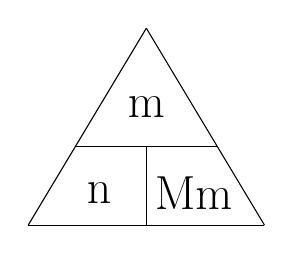
\begin{tikzpicture}
        \draw (0,2.5)--(1.5,0);
        \draw (1.5,0)--(-1.5,0);
        \draw (-1.5,0)--(0,2.5);
        \draw (0,1.0)--(0,0);
        \draw (-0.9,1)--(0.9,1);
        \node at (0,1.5) {\LARGE m};
        \node at (-0.6,0.4) {\LARGE n};
        \node at (0.6,0.4) {\LARGE Mm};
    \end{tikzpicture}    
\end{center}
Vi skal nå teste ut dette med noen oppgaver.\\\\
\textbf{Oppgaver:}\\

\noindent Hvor mange gram har vi av stoffene $NH_4Cl, NaOH, HCl, H_2SO_4, NH_3, H_3PO_4$ og$ CO_2$ når vi har 2,2mol?\\\\
\textbf{Hint:} om vi bruker trekanten så er vi at:
$$m=n\cdot Mm$$
Først beregner vi Mm($NH_4Cl)$:
$$Mm(NH_4Cl)=14,0g/mol+4\cdot 1,01g/mol+35,45g/mol=53,49g/mol$$\\
Antall gram blir da:\\
$$m=n(NH_4Cl)\cdot Mm(NH_4cL)=2,2mol\cdot 53,49g/mol=117,68g$$\\\\
Nå kan du fullføre for de andre stoffene.\\\\
Hvor mange mol har vi av stoffene $NH_4Cl, NaOH, HCl, H_2SO_4, NH_3, H_3PO_4$ og $CO_2$ når vi har 34g?\\\\
\textbf{Hint:}Om du bruker trekanten får du:
$$n=\frac{m}{Mm}$$
Først beregner vi Mm($NH_4Cl)$:
$$Mm(NH_4Cl)=14,0g/mol+4\cdot 1,01g/mol+35,45g/mol=53,49g/mol$$\\
Antall mol blir da:
$$n(NH_4Cl)=\frac{m(NH_4Cl)}{Mm(NH_4Cl)}=\frac{34g}{53,49g/mol}=0,64mol$$\\
Nå kan du fullføre for de andre stoffene.\\\\
\begin{center}
    \textbf{Støkiomteriske beregninger:}
\end{center}\vspace{1cm}
Støkiometriske beregninger er \textbf{mengdebaserte beregninger} i kjemi som handler om \textbf{forholdet mellom stoffer i en kjemisk reaksjon}. Navnet kommer fra “støkiometri”, som betyr “måling av elementer”.\\\\
\textbf{Kort sagt:} det dreier seg om \textbf{å finne hvor mye av et stoff som reagerer eller dannes} basert på den kjemiske reaksjonslikningen.
\textbf{Hva støkiometriske beregninger ofte brukes til:}
\begin{enumerate}
    \item Finne hvor mye reaktant som trengs.
    \item Finne hvor mye produkt som dannes.
    \item Bestemme begrensende reaktant.   
\end{enumerate}
Vi skal nå se på disse.\newpage
\noindent\textbf{1 finne hvor mye reaktant som trengs:}\\\\
Når karbon forbrenner dannes det karbondioksid:\\\\
$$C+O_2=CO_2$$
En slik kjemisk reaksjon forteller oss hvor mange enheter som deltar i reaksjonen:\\
$$1\:C atom+1O_2\:molekyl=1CO_2\:molekyl$$
Her kan vi egentlig "gange" på hver side med Avogadros tall ($N_A=6,022\cdot 10^{23}$). Og da kan vi faktisk skrive:
$$1\:mol\:C+\:1mol\:O_2=1\:mol\:CO_2$$

\noindent La oss si at vi skal produsere 234g $CO_2$. Hvor mye C og $O_2$ trenger vi da? \\
Det er ikke så enkelt å forstå det, men det er her antall mol blir veldig viktig.  Vi beregner først hvor mange mol $CO_2$ vi har når vi har 234g $CO_2$.  Den molare massen til $CO_2$ er $Mm(CO_2)=12,0g/mol+2\cdot 16,0g/mol=44,0g/mol$.  Antall mol beregnes etter følgende formel (bruk trekanten om du er usikker):\\
$$n(CO_2)=\frac{m(CO_2)}{Mm(CO_2)}=\frac{234g}{44g/mol}=5,318mol$$\\
Nå skal vi lage en oversiktstabell for reaksjonen:


\begin{table}[h!]
    \centering
    \begin{tabular}{cccccc}
         R.x.:&  C&  +&  $O_2$&  =& $CO_2$\\
         molforhold:&1  &  & 1 &  &1 \\
         &  &  &  &  & \\
    \end{tabular}
\end{table}
Dette betyr at 1 mol C reagerer med 1 mol $O_2$ og vi får laget 1 mol $CO_2$.  Men vi ønsker å få laget 5,31mol $CO_2$.  Da må vi endre 1 tallet under $CO_2$ ved å enten gange eller dele.\newpage  
Her ganger vi, og vi får:
\begin{table}[h!]
    \centering
    \begin{tabular}{cccccc}
         R.x.:&  C&  +&  $O_2$&  =& $CO_2$\\
         molforhold:&1  &  & 1 &  &1 \\
         $\cdot 5,318$&$1\cdot 5,318mol$  & &  $1\cdot 5,318mol$&  &$1\cdot 5,318mol$ \\
         i gram:&$12g/mol\cdot 5,318mol$  & &  $32g/mol\cdot 5,318mol$&  &$44g/mol\cdot 5,318mol$ \\
         i gram:&$63,816g$  & &  $170,176g$&  &$233,992g$ \\
         Massebalanse:&$63,816g$  & +&  $170,176g=233,992g$&  &$233,992g$ \\
    \end{tabular}
\end{table}\\
\textbf{Viktig poeng:} Vi ser at masen før reaksjon er lik massen etter.  Dette stemmer med loven om bevaring av masse.  Den sier at \textbf{den totale massen av stoffene som deltar i en reaksjon er den samme før og etter reaksjonen} – selv om stoffene endrer form, bindinger eller tilstand. \\\\
\textbf{2 Finne hvor mye produkt som dannes:}\\
Hvor mye $CO_2$ dannes ved forbrenning av 1245kg C?\\
Nå skal vi først lage en oversiktstabell for reaksjonen:


\begin{table}[h!]
    \centering
    \begin{tabular}{cccccc}
         R.x.:&  C&  +&  $O_2$&  =& $CO_2$\\
         molforhold:&1  &  & 1 &  &1 \\
         &  &  &  &  & \\
    \end{tabular}
\end{table}
Dette betyr at 1 mol C reagerer med 1 mol $O_2$ og vi får laget 1 mol $CO_2$. Vi må først finne ut hvor mange mol C vi har.  Hint: 1245kg=1245000g\\\\
Vi beregner antall mol C:\\\\
$n(C)=\frac{1245000g}{12g/mol}=103750mol$\\\\
Da må vi endre 1 tallet under $C$ ved å enten gange eller dele.  Her ganger vi, og vi får:
\begin{table}[h!]
    \centering
    \begin{tabular}{cccccc}
         R.x.:&  C&  +&  $O_2$&  =& $CO_2$\\
         molforhold:&1  &  & 1 &  &1 \\
         $\cdot 103750$&$1\cdot 103750mol$& &  $1\cdot 103750mol$&  &$1\cdot 103750mol$\\
         i gram:&$12g/mol\cdot 103750mol$& &  $32g/mol\cdot 103750mol$&  &$44g/mol\cdot 103750mol$\\
         i gram:&$1245000g$& &  $3320000g$&  &$4565000g$\\
         Massebalanse:&$1245000g$& +&  $3320000g=4565000g$&  &$4565000g$\\
    \end{tabular}
\end{table}\newpage
 


\newpage
Hvor mange gram C og $O_2$  trenger vi for å lage 500g $CO_2$?\\\\
Antall mol $CO_2$: $n(CO_2)=\frac{500g}{44g/mol}=11,364mol$ 
\begin{table}[h!]
    \centering
    \begin{tabular}{cccccc}
         R.x.:&  C&  +&  $O_2$&  =& $CO_2$\\
         molforhold:&$1\cdot 11,364$  &  & $1\cdot 11,364$ &  &$1\cdot 11,364$ \\
         masse:&$11,364mol\cdot 12g/mol$&  &$11,364mol\cdot 32g/mol$ &  &$11,364mol\cdot 12g/mol$\\
          masse:&$136,416$& + &$363,776g=500,192$ &  &$500,192g/mol$\\
    \end{tabular}
\end{table}\\
Vi tar utgangspunkt i reaksjonen
$$C+O_2=CO_2$$\\
1. Hvor mye får vi dannet av $CO_2$ om vi har 456g $O_2$?\\
2. Hvor mye får vi dannet av $CO_2$ om vi har 456g $C$?\\
3. Hvor mye trenger vi av C og $O_2$ om vi ønsker 456g $CO_2$?\\\\
Rekkefølgen for å løse slik oppgaver:\\
1. bestem antall mol av stoffet du har fått oppgitt i gram.
2. lag skjema og finn antall mol.\\
3. regn om til gram.\\\\
1. 456g $O_2$:\\\\
Antall mol $O_2$:  $n(O_2)=\frac{m(O_2)}{Mm(O_2)}=\frac{456g}{32g/mol}=14,25mol$\\\\
Vi setter opp reaksjonsskjema:\\\\
\begin{table}[h!]
    \centering
    \begin{tabular}{cccccc}
         R.x.:&  C&  +&  $O_2$&  =& $CO_2$\\
         molforhold:&$1\cdot 14,25$  &  & $1\cdot 14,25$ &  &$1\cdot 14,25$ \\
         masse:&$14,25mol\cdot 12g/mol$&  &$14,25mol\cdot 32g/mol$ &  &$14,25mol\cdot 44g/mol$\\
          masse:&$171g$& + &$456g=627g$ &  &$627$\\
    \end{tabular}
\end{table}\\
\newpage
\textbf{Oppgaver:}\\
Gitt følgende r.x.:
$$2H_2+O_2=2H_20$$\\
1. Hvor mye vann får laget om  vi starter med 324g $H_2$?\\
1. Hvor mye vann får laget om  vi starter med 324g $O_2$?\\
1. Hvor trenger vi av $H_2$ og $O_2$  vi får dannet 324g $H_2O$?\\

  \noindent\textbf{3 Bestemme begrensende reaktant:}\\\\
    En artig reaksjon er forbrenning av hydrogen ($H_2)$.  Det er den som skjer i en hydrogenbil:\\\\
$$2H_2(g)+O_2(g)=2H_2O(g)+ el. energi$$\\
Vi lar 234g $H_2$ reagere med 850g $O_2$.  Hvor mye vann får vi laget?\\\\
Her må vi først beregne antall mol av hvert stoff:\\\\\\
$n(H_2)=\frac{m(H_2)}{Mm(H_2)}=\frac{234g}{2,02g/mol}=115,842mol$\\\\\\
$n(O_2)=\frac{m(O_2)}{Mm(O_2)}=\frac{850g}{32,00g/mol}=89,279mol$\\\\
Så må vi set på hva dette betyr.  Er det mulig at alt blir brukt av begge stoffene?  Vi setter opp skjmeaet for reeaksjonen:\\
\begin{table}[h!]
    \centering
    \begin{tabular}{cccccc}
         R.x.:&  $2H_2(g)$&  +&  $O_2(g)$&  =& $2H_2O(g)$\\
         molforhold:&$2$  &  & $1$ &  &$2$ \\
                   
    \end{tabular}
\end{table}\\
Her ser vi at vi at dobbelt så mange mol $H_2$ reagerer med $O_2$.  2 mol $H_2$ reagerer med 1 mol $O_2$. Nå kommer det som er vanskelig. Vi har 115,842mol $H_2$.  Foran $H_2$ står det 2. VI sakel endre 2 til 115,842 ved å kun bruke "gange" og "dele".  Da bruek vi "veien om 1".\newpage 
Vi deler på 2 og får 1, og så ganger med 115,842:\\
\begin{table}[h!]
    \centering
    \begin{tabular}{cccccc}
         R.x.:&  $2H_2(g)$&  +&  $O_2(g)$&  =& $2H_2O(g)$\\
         molforhold:&$\frac{2\cdot 115,842}{2}$  &  & $\frac{1\cdot 115,842}{2}$ &  &$\frac{2\cdot 115,842}{2}$ \\
         molforhold:&115,842& &57,921&&115,842
                   fdf
    \end{tabular}
\end{table}\\

 \end{document}